\documentclass[10pt, a4paper]{article}
\usepackage{amsmath}  % improve math presentation
\usepackage{graphicx} % takes care of graphic including machinery
\usepackage[a4paper, top=2.5cm, bottom=2.5cm, left=2.2cm, right=2.2cm]{geometry}
\usepackage{listings}
\usepackage{color} %red, green, blue, yellow, cyan, magenta, black, white
\usepackage{tcolorbox}

%%%%%%%%%%%%%%%%%%%%%%%%%%%%%%%%%%%%%%%%%%%%%%%%%%%%%%%%%%%%%%%%%%%%%%%%%%%%%%%%%%%%%%%%%%%%%%%%%%%%%%%%%%
\lstset{basicstyle=\ttfamily, breaklines = true, tabsize=2}
\graphicspath{ {./Images/} }
\setlength{\parskip}{1em}
%%%%%%%%%%%%%%%%%%%%%%%%%%%%%%%%%%%%%%%%%%%%%%%%%%%%%%%%%%%%%%%%%%%%%%%%%%%%%%%%%%%%%%%%%%%%%%%%%%%%%%%%%%
\begin{document}
%%%%%%%%%%%%%%%%%%%%%%%%%%%%%%%%%%%%%%%%%%%%%%%%%%%%%%%%%%%%%%%%%%%%%%%%%%%%%%%%%%%%%%%%%%%%%%%%%%%%%%%%%%
\title{
    Mathematics - Numerical Analysis \\ \large Problem Sheet 0: Trapezoid Rule}
\author{Xin Wang}

\maketitle
%%%%%%%%%%%%%%%%%%%%%%%%%%%%%%%%%%%%%%%%%%%%%%%%%%%%%%%%%%%%%%%%%%%%%%%%%%%%%%%%%%%%%%%%%%%%%%%%%%%%%%%%%%
\section{Trapezoid Rule}

Not every integral has an exact solution. To approximate a solution we can employ numerical
techniques, the simplest of which is the Trapezoidal Rule. Consider the integral of $f(x)$ over the
interval[a,b] begin by dividing the interval into $n$ segments of equal length $h = \frac{b-a}{n}$.
\begin{figure} [h!]
    \centering
    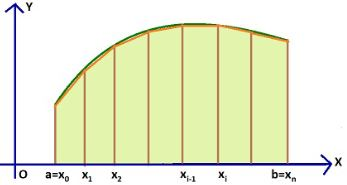
\includegraphics[scale=0.6]{Trapezoid.JPG}
\end{figure}

\begin{enumerate}
    \item Set $a=x_0$ and $b=x_n$, then the $n$ intervals are $[x_i,x_{i+1}]$ for $i=0\dots n-1$. The area
    under the curve $f(x)$ now consists of integrating over each segment and summing:
    $$
        \int_{x_i}^{x_{i+1}}f(x) \: dx
    $$

    \item For each segment, approximate the integral with the area of a trapezoid of left height $f(x_i)$and
    right height $f(x_{i+1})$, giving an approximate area:
    $$
        \int_{x_i}^{x_{i+1}}f(x) \: dx \approx \frac{1}{2}h[f(x_i)+f(x_{i+1})]
    $$

    \item To see a simple case, let $n=3$, so $a=x_0$ and $b=x_3$:
    $$
        \frac{1}{2}h[f(x_0)+f(x_{1})] + \frac{1}{2}h[f(1)+f(x_{2})] + \frac{1}{2}h[f(2)+f(x_{3})]
    $$
    which can be tidied up as:
    $$
        \frac{1}{2}h[f(x_0)+2f(x_1)+2f(x_2)+f(x_3)]
    $$
\end{enumerate}

\begin{tcolorbox}[colback=white]
    The general case is defined as: 
    $$
        I_n = \int_a^b f(x) \approx \left(\frac{b-a}{2n}\right)\left[f(x_0)+2\left(\sum_{i=1}^{n-1}f(x_i)\right)+f(x_n)\right]
    $$
    where $x_0 = a$, $x_1 = \frac{1}{n}$, $x_2 = 2 \times \frac{1}{n}$, $\dots$, $x_n = b$
\end{tcolorbox}

\begin{align*}
    I_4 &= \left(\frac{1-0}{2*4}\right)\left[\exp(0)+2\left[\exp(\frac{1}{4})\right]+2\left[\exp(2\times\frac{1}{4})\right]+2\left[\exp(3\times\frac{1}{4})\right]+\exp(1)\right]
\end{align*}

%%%%%%%%%%%%%%%%%%%%%%%%%%%%%%%%%%%%%%%%%%%%%%%%%%%%%%%%%%%%%%%%%%%%%%%%%%%%%%%%%%%%%%%%%%%%%%%%%%%%
\section{Exercise 1}

\begin{itemize}
    \item Use the Trapezoidal Rule to obtain:
    $$
        I=\int_0^1 e^x dx = e - 1 \approx 1.718281828
    $$
    where $I_n$ is the approximate solution with $n$ segments 
    \begin{enumerate}
        \item Begin by obtaining $I_4$.
        \item Increase $n$ to improve precision.
        \item Let $\epsilon_n$ be the error made with segment length $h=\frac{(b-a)}{n}$. For each
        $n$, calculate $\epsilon_n=|I-I_n|$.
    \end{enumerate}
    \item Tabulate results and compare $n$ and the error $\epsilon_n$. Is there any relationship
    between the error and the number of segments? 
    \item Write a simple Matlab code to investigate this:
    \begin{itemize}
        \item Given a function $f(x)$, an interval $[a,b]$ and a number of segments $n$, your code
        should integrate the function numerically over $[a,b]$ with the interval divided
        into $n$ segments. Compare with the exact solution. 
        \item Next, incorporate the code written into a loop to investigate the effect of increasing
        $n$ on the error. Integrate for $n=2...N$ where $N$ is chosen to be suitably large. Plot the
        error against $n$. Try a log-log plot for $\epsilon_n$ and $h$, what is the conclusion?
        \item Test this on several functions and intervals.
    \end{itemize}
\end{itemize}

%%%%%%%%%%%%%%%%%%%%%%%%%%%%%%%%%%%%%%%%%%%%%%%%%%%%%%%%%%%%%%%%%%%%%%%%%%%%%%%%%%%%%%%%%%%%%%%%%%%%%%%%%%
\section{Exercise 2}

Now consider Simpson’s rule which is a refinement of the trapezoidal rule. Take $n$ - an even number and proceed as follows:
\begin{align*}
    \int_a^b f(x)\: dx \approx \left(\frac{b-a}{3n}\right)\left[f(x_0)+2\left(\sum_{i=1}^{\frac{n}{2}-1}f(x_{2i})\right)+4\left(\sum_{i=1}^{\frac{n}{2}}f(x_{2i-1})\right)+f(x_n)\right]
\end{align*}

To understand the rule, let $n=6$:
\begin{align*}
    \frac{h}{3}\left[f(x_0)+4f(x_1)+2f(x_2)+4f(x_3)+2f(x_4)+4f(x_5)+f(x_6)\right]
\end{align*}

\begin{enumerate}
    \item Repeat the previous exercise and error analysis with Simpson’s rule.
    \item What are the observations?
    \item 
\end{enumerate}
\end{document}